\section{Bermuda Vertex-Centric Node++} 
As discussed in Section \ref{sec:EC}, the Bermuda-EC algorithm assumes that the core messages can fit in the memory of a single reducer. However, it is not always guaranteed to be the case, especially in web-scale graphs.

One crucial observation is that the access pattern of the pivot messages
can be learned and leveraged for better re-usability. 
In MapReduce, a single reduce instance processes many keys (graph nodes) in a specific sequential order. This order is defined based on the key comparator function. 
For example, let $h()$ be the key partitioning function and $l()$ be key comparator function within the MapReduce framework, 
then $h(u)=h(w)=i$ and $l(u,w)<0$ implies that the reduce instance $R_i$ is responsible for the computations over nodes $u,~w$, and also the computations 
of node $u$ precede   that of node $w$. 
Given these known functions, the relative order among the keys in the same reduce instance becomes known,
 and the access pattern of  the pivot message can be predicted. 
The knowledge of the access pattern of the pivot messages holds a great promise for proving better caching and better memory utilization.

Inspired by these facts, we propose the~Bermuda-VC algorithm which supports random access 
over the pivot messages by caching them in main-memory while streaming in the core messages. 
More specifically, Bermuda-VC will reverse the assumption of Bermuda-EC, where we now try to make the pivot messages arrive first to reducers, 
get them cached and organized in memory, and then the core messages are received and processed against the pivot messages. 
Although the size of the pivot messages is usually larger than that of the core messages,  
their access pattern is more predictable which will enable better caching strategies as we will present in this section. 
%Moreover, \Bermuda-VC maintains the independence of distinct key/node's reduce computation as MR-Baseline algorithm. 
The Bermuda-VC algorithm is presented in Algorithm \ref{alg:Bermuda-VC}. 
\begin{algorithm}[t!]
	\begin{algorithmic}[1]
			\item[] \textbf{Map}: Input:($ \langle v;(N_v^L ,N_v^H) \rangle$) 
            \item[] {Let $h(.)$ be a key partitioning function into [0,k-1] }
            \item[] {Let $l(.)$ be a key comparator function}
			\STATE emit $\langle v;(v,N_v^L,N_v^H) \rangle$
			\STATE \emph{Group} the set of nodes in $N_v^H$ by $h(.)$
			\FORALL {$i \in [0,k-1]$}
				\IF {$gp_i \neq \emptyset$}
                	\STATE $gp_i \Leftarrow sort(gp_i) based on l(.)$
                    \STATE $u \Leftarrow gp_i.first$
					\STATE $AP_{v,i} \Leftarrow accessPattern(gp_i)$
					\STATE emit $\langle u;(v,AP_{v,i},N_v^H) \rangle$
				\ENDIF
			\ENDFOR
            \item[]
			\item[] \textbf{Reduce}:Input:$[\langle u;(v,AP_{v,i},N_v^H) \rangle]$ 
			\STATE initiate the core node $u$' $N_u^L,N_u^H$ in main memory
            \FORALL {pivot message $\langle u;(v,AP_{v,i},N_v^H) \rangle $}
            	\FORALL{$w \in N_v^H \bigcap N_u^H$}
                	\STATE emit $\triangle_{vuw}$
                \ENDFOR
                \STATE {Put $(v,AP_{v,j},N_v^H)$ into shared buffer}
                \STATE {$N_u^L\leftarrow N_u^L-\lbrace v \rbrace$}
            \ENDFOR
            \FORALL {$r \in N_u^L$}
            	\STATE {Fetch $(r,AP_{r,i},N_{r}^H)$ from shared buffer}
         		\FORALL{$w \in N_{r}^H \bigcap N_u^H$}
                	\STATE emit $\triangle_{ruw}$
               	\ENDFOR
            \ENDFOR
	\end{algorithmic}
	\caption{Bermuda-VC}
	\label{alg:Bermuda-VC}
\end{algorithm}
\begin{figure}[t]
		\centering	
		\includegraphics[scale=0.4]{figures/bermuda/BNode++.eps}
		\caption {Bermuda-VC Execution.}
		\label{fig:Bermuda-VC}
\end{figure}

% The high level idea of \Bermuda-VC algorithm is
The Bermuda-VC algorithm uses a shared buffer for  caching the pivot messages.
% Based on message sharing management, the general approach of its reduce computation is similar to MR-Baseline algorithm. 
And then, for the reduce-side computations over a core node $u$, the reducer compares $u$'s core message with all related pivot messages---some are associated with $u$'s core message, while the rest should be residing in the shared buffer. 
%
Bermuda-VC algorithm applies the same scheme to avoid generating redundant pivot messages. It utilizes a universal key partitioning function to group effective neighbors $N_v^H$ of each node $v$. 
In order to guarantee the availability of the pivot messages, a universal key comparator function is utilized to sort the destination nodes in each group (Line 5, Algorithm \ref{alg:Bermuda-VC}). As a result, destination nodes are sorted based on their processing order. The first node in group $gp_i$ indicates the earliest request of a pivot message. 
Hence, each node $v$ sends a pivot message to the first node of each non-empty group by emitting key value pairs where key equals the first node ID (Lines 6-8, Algorithm \ref{alg:Bermuda-VC}). 

Combined with the sorting phase of the MapReduce framework, Bermuda-VC guarantees the availability of all needed pivot messages of any node $u$ when $u$'s core message is received by a reducer, i.e.,  the needed pivot messages are either associated with $u$ itself or associated with another nodes processed before $u$. 

The reducers' processing mechanism is similar to that of  the MR-Baseline algorithm. 
Each node $u$ reads its core message for initiating $N_u^H$ and $N_v^L$ (Line 9), and then it iterates over every pivot message associated with key $u$ against its effective adjacency list $N_v^H$ to enumerate the triangles (Lines 10-12). As discussed before, not all expected pivot messages are carried with key $u$. 
The rest of the related pivot messages reside in the shared buffer. Here, $N_v^L$ is used for fetching the rest of these pivot 
messages (Line 14, Algorithm \ref{alg:Bermuda-VC}), and enumerating the triangles (Lines 15-18, Algorithm \ref{alg:Bermuda-VC}). 
Moreover, the new coming pivot messages associated with node $u$ are pushed into the shared buffer for further access by other nodes (Line 13). 
Figure \ref{fig:Bermuda-VC} illustrates the reduce-side processing flow of Bermuda-VC. 
In the following sections, we will discuss in more details the management of the pivot messages in the shared buffer.
%Its appeal stems from the fact that the reduce computation of different keys/nodes is isolated. While, it requires random access to pivot messages which may not fit in main-memory for massive graphs. To solve this problem, we introduce different message sharing management schemes as described next. 

\subsection{Message Sharing Management}
Note that, each reduce instance uses its shared buffer to organize sharing pivot messages in memory. Message sharing via shared buffer is effective because the reduce computation program access the same pivot message over and over. By keeping as much of  pivot message as possible in the shared buffer, it avoids access the slower medium--disk. 
In general, there are two types of operations over the shared buffer inside a reduce instance, which are: {\em ``Put''} for adding new incoming pivot messages into the shared buffer (Line 13), and {\em ``Get''} for retrieving  the needed pivot messages (Lines 15-18).  For massive graphs, the main memory may not hold all the pivot messages.  
This problem is similar to the classical caching problem studied in~\cite{keramidascache2007, petoumenos2009}, where a {\em  reuse-distance} factor is used to estimate the distances between consecutive references of a given cached element, and based on that effective  replacement policies can be deployed. We adopt the same idea in  Bermuda-VC.

Interestingly, in addition to the reuse distance, all access patterns of each pivot message can be easily estimated in our context.
The access pattern $AP$ of a pivot message is defined as the sequence of graph nodes (keys) that will reference this message. 
In particular, the access pattern of a pivot message from node $v$ to reduce instance $R_i$ can be computed based on the sorted effective nodes $gp_i$ received by $R_i$. Several interesting metrics can be derived from this access pattern. 
For example, the first node in $gp_i$ indicates the occurrence of the first reference, the size of $gp_i$ equals the cumulative reference frequency. 
Such access pattern information is encoded within each pivot message (Lines 7-8, Algorithm \ref{alg:Bermuda-VC}). 
With the availability of this access pattern, effective message sharing strategies can be deployed under limited memory.  

\begin{figure}[t]
		\centering	
		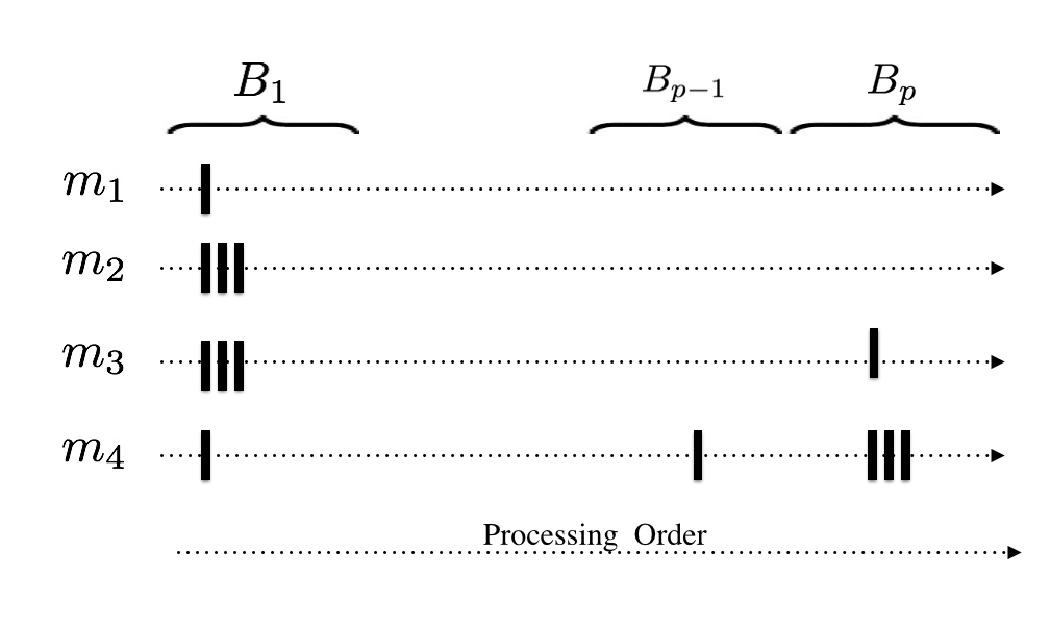
\includegraphics[scale=0.4]{figures/bermuda/usagePattern.eps}
		\caption {Various access Patterns for Pivot Messages.}
		\label{fig:upattern}
\end{figure}

As an illustrative example, Figure \ref{fig:upattern} depicts different access patterns for four pivot messages \{$m_1,~m_2,~m_3,~m_4$\}. 
The black bars indicate requests to the corresponding pivot message, while the gaps represent the re-use distances (which are idle periods for this message). 
Pivot messages may exhibit entirely different access patterns, e.g., pivot message $m_1$ is referenced only once, while others are utilized more than once, and some pivot messages are used in dense consecutive pattern in a short interval, {\eg}, $m_2$ and $m_3$. 
%
Inspired by these observations, we propose two heuristic-based replacement policies, namely \emph{usage-based tracking}, and \emph{bucket-based tracking}. 
They trade off the tracking overhead with memory hits as will be described next. 


\hspace{-2em}
\textbf{$\bullet$Usage-Based Tracking}
Given a pivot message originated from node $v$, the total use frequency is limited to $\sqrt[]{m}$, referring to the number of its effective neighbors, which is much smaller than the expected number of nodes processed in a single reducer, which is estimated to $n/k$. This  implies that each pivot message may become useless (and can be discard) as a reducer progresses, and it is always desirable to detect the earliest time at which a pivot message can be discarded to maximize the  memory's utilization.

The main idea of the usage-based tracking is to use a usage counter per pivot message in the shared buffer. And then, the tracking is performed as follows. Each \emph{Put} operation sets the counter as the total use frequency. And, only the pivot messages whose usage counter is larger than zero are added to the shared buffer. Each \emph{Get} operation decrements the counter of the target pivot message by one. Once the counter reached zero, the corresponding pivot message is evicted from the shared buffer. 

The usage-based scheme may fall short in optimizing sparse and scattered access patterns. For example, as shown in Figure~\ref{fig:upattern}, the reuse distance of message $m_4$ is large. Therefore, the usage-based tracking strategy has to keep $m_4$ in the shared buffer although it will not be referenced for a long time. What's worse, such  scattered access is common in massive graphs. Therefore,  pivot messages may unnecessarily overwhelm the available memory of each single reduce instance.  

\hspace{-2em}
\textbf{Bucket-Based Tracking}
We introduce the \emph{Bucket-based} tracking strategy to optimize message sharing over scattered access patterns. The main idea is to manage the access patterns of each pivot message at a smaller granularity, called a {bucket}. The processing sequence of keys/nodesis sliced into buckets as illustrated in Figure \ref{fig:upattern}. 
In this work, we use the range partitioning method for balancing workload among buckets. 
Correspondingly, the usage counter of one pivot message is defined per bucket, i.e., each message will have an array of usage counters of a length equals to the number of its buckets. 
For example, the usage count of $m_4$ in the first bucket is $1$ while in the second bucket is $0$. 
Therefore, for a pivot message that will remain idle (with no reference) for a long time, its counter array will have a long sequence of adjacent zeros. Such access pattern information can be computed in the map function, encoded in access pattern (Line 7 in Algorithm~\ref{alg:Bermuda-VC}), and passed to the reduce side. 

\begin{figure}[t]
		\centering	
		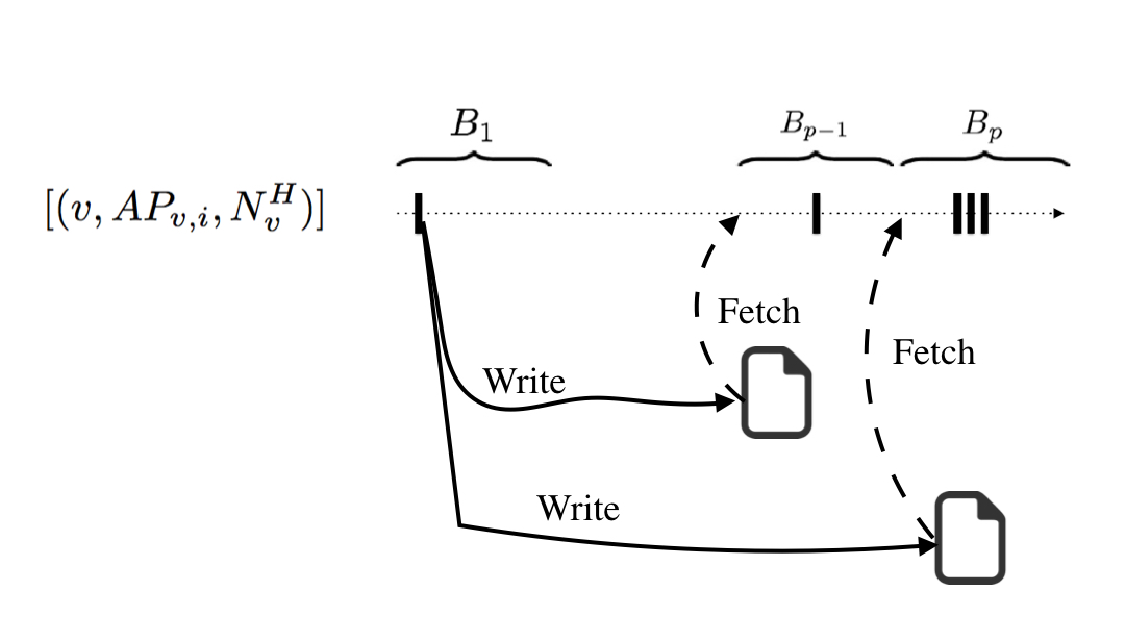
\includegraphics[scale=0.4]{figures/bermuda/bucketFetching.eps}
		\caption {Read and Write Back-up files}
		\label{fig:bucketFetch}
\end{figure}

The corresponding modification of the \emph{Put} operation is as follows.  Each new pivot message will be pushed into the shared buffer (in memory) and backed up by local files (in disk) based on its access pattern. 
Figure \ref{fig:bucketFetch} illustrates this procedure. For the arrival of a pivot message with the access pattern $[1,0,.., 1,3]$, the reduce instance actively adds this message into back-up files for buckets $B_{p-1}$ (next-to-last bucket) and $B_{p}$ (last bucket). And then, at the end of each bucket processing and before the start of processing the next bucket, 
all pivot messages in the shared buffer are discarded, and a new set of pivot messages is fetched from the corresponding back-up file into memory(See Figure \ref{fig:bucketFetch}). 

The Bucket-based tracking strategy provides better memory utilization since it prevents the long retention of unnecessary pivot messages. In addition, usage-based tracking  can be applied to each bucket to combine both benefits,  which is referred to as the {\em bucket-usage} tracking strategy. 

\subsection{Disscussion}
In this section, we show the benefits of the Bermuda-VC algorithm over the Bermuda-EC algorithm. 
Furthermore, we discuss the effect of  parameter $p$, which is the the number of buckets, on the performance.

Under the same settings of the number of reducers $k$, the Bermuda-VC algorithm generates more intermediate message and takes longer execution time.  Firstly, the Bermuda-VC algorithm generates the same number of pivot messages while generating more core messages ({\ie}, additional $N_v^L$ for reference in the reduce side).
Thus, the total size of the extra $N_v^L$ core message is $\sum_{v \in V} N_v^L=m$. 
Such noticeable size of extra core messages requires additional time for generating and shuffling. 
Moreover, an additional computational overhead (Lines 13-14) is required for the message sharing management. 

However, because of the proposed sharing strategies, the Bermuda-VC algorithm can work under smaller settings for $k$---which are settings under which the Bermuda-EC algorithm will probably fail.  In this case, the benefits brought by having a smaller $k$  will exceed the corresponding cost. In such cases, Bermuda-VC algorithm will outperform Bermuda-EC algorithm. 

Moreover, compared to the disk-based Bermuda-EC algorithm, the Bermuda-VC algorithm has a relatively smaller disk I/O cost because the predictability of the access pattern of the pivot messages, which enable purging them early, while that is not applicable to the core messages. Notice that, for any given reduce instance, the expected usage count of pivot message from $u$ is $d_u^H/k$. Thus, the expected usage count for any pivot message is $E(d_u^H)/k$, equals $m/nk$.  Therefore, the total disk I/O with pivot messages is at most $m^2/nk$, smaller than disk I/O cost of Bermuda-EC algorithm $m^2/Mk$, where $M$ stands for the size of the available memory in a single machine.

{\textbf{ Effect of the number of buckets $p$: }} At a high level, $p$ trades off the space used by the shared buffer with the I/O cost for writing and reading the back-up files. Bermuda-VC algorithm favors smaller settings of $p$ in the capacity of main-memory. As $p$ decreases, the expected number of reading and writing decreases, however the total size of the pivot messages in the shared buffer may exceed the capacity of the main-memory. 
For a setting of $p$, the expected size of the pivot messages for any bucket is $O(m/kp)$. Therefore, a visible solution for $O(m/kp) \le M$ is $ \ge O(m/kM)$. 
Here, $p$ is set as $O(m/kM)$ where $m$ is the size of the input graph, and $M$ is the size of the available memory in a single machine. 

